
\documentclass[uplatex, dvipdfmx]{jsarticle}

\usepackage{amsmath,amssymb,amsthm,mathtools}
\usepackage{tikz}
\usetikzlibrary{decorations.pathreplacing,calc,arrows.meta,patterns}
\usepackage{pgfplots}
\pgfplotsset{compat=1.18}
\usepackage{tcolorbox}
\tcbuselibrary{theorems}

\newtcbtheorem[number within=section]{definition}{定義}{
  colback=blue!5, colframe=blue!40!black, fonttitle=\bfseries
}{def}
\newtcbtheorem[use counter from=definition]{proposition}{命題}{
  colback=green!5, colframe=green!35!black, fonttitle=\bfseries
}{prop}
\newtcbtheorem[use counter from=definition]{theorem}{定理}{
  colback=red!5, colframe=red!40!black, fonttitle=\bfseries
}{thm}
\newtcbtheorem[use counter from=definition]{remark}{注意}{
  colback=yellow!5, colframe=yellow!40!black, fonttitle=\bfseries
}{rem}
\newtcbtheorem[use counter from=definition]{example}{例}{
  colback=gray!5, colframe=gray!50!black, fonttitle=\bfseries
}{ex}
\tcolorboxenvironment{proof}{
  colback=white, colframe=black!20,
  leftrule=2pt, rightrule=0pt, toprule=0pt, bottomrule=0pt
}

\newcounter{algcounter}
\newtcolorbox{algorithm}[1]{
  colback=white, colframe=black!70,
  fonttitle=\bfseries, title={Algorithm~\refstepcounter{algcounter}\thealgcounter\label{#1}},
  boxrule=0.8pt
}

\begin{document}

最適輸送理論は，ある確率分布を別の確率分布へ移すための最小コストを求める問題を扱う．
本稿では，Monge (1781) による原初的な定式化から出発し，
Kantorovich (1942) による緩和とその双対理論までを展開する．

%% ==========================================================
%%  第1節：Monge 問題
%% ==========================================================
\section{Monge 問題}

確率分布の再配置を最適化する問題は，
フランスの数学者 Monge が土木工学の文脈で提起したことに始まる．
与えられた二つの確率分布に対し，
一方を他方へ移すための最小費用を達成する写像を求めることが目標である．
この問題を正確に記述するために，まず必要な概念を導入する．

\begin{definition}{$\sigma$加法族}{sigma_algebra}
集合 $X$ の部分集合族 $\mathcal{A}\subset 2^X$ が
\textbf{$\sigma$加法族}（$\sigma$-algebra）であるとは，
次の三条件を満たすことをいう：
\begin{enumerate}
  \item $X\in\mathcal{A}$，
  \item $A\in\mathcal{A}$ ならば $A^c\in\mathcal{A}$，
  \item $A_1,A_2,\ldots\in\mathcal{A}$ ならば
        $\bigcup_{n=1}^{\infty}A_n\in\mathcal{A}$．
\end{enumerate}
\end{definition}

\begin{definition}{可測空間}{measurable_space}
集合 $X$ とその上の $\sigma$加法族 $\mathcal{A}$ の組
$(X,\mathcal{A})$ を\textbf{可測空間}と呼ぶ．
$\mathcal{A}$ の元を\textbf{可測集合}という．
\end{definition}

\begin{definition}{測度}{measure}
可測空間 $(X,\mathcal{A})$ 上の\textbf{測度}とは，
関数 $\mu\colon\mathcal{A}\to[0,\infty]$ であって次を満たすものをいう：
\begin{enumerate}
  \item $\mu(\emptyset)=0$，
  \item 互いに素な可測集合の列 $A_1,A_2,\ldots\in\mathcal{A}$
        （$A_i\cap A_j=\emptyset$, $i\neq j$）に対し
        \[
          \mu\!\left(\bigcup_{n=1}^{\infty}A_n\right)
          =\sum_{n=1}^{\infty}\mu(A_n)
        \]
        が成り立つ（$\sigma$加法性）．
\end{enumerate}
組 $(X,\mathcal{A},\mu)$ を\textbf{測度空間}という．
特に $\mu(X)=1$ を満たす測度を\textbf{確率測度}と呼ぶ．
\end{definition}

\begin{definition}{可測写像}{measurable_map}
$(X,\mathcal{A})$，$(Y,\mathcal{B})$ を可測空間とする．
写像 $T\colon X\to Y$ が\textbf{可測写像}であるとは，
任意の $B\in\mathcal{B}$ に対し $T^{-1}(B)\in\mathcal{A}$ が成り立つことをいう．
\end{definition}

測度論では，集合の「大きさ」は $\sigma$加法族に属する集合に対してのみ定まる．
写像 $T$ を通じて $Y$ 側の集合 $B$ を $X$ 側で扱うには，
逆像 $T^{-1}(B)$ が $X$ の $\sigma$加法族 $\mathcal{A}$ に属する必要がある．

\begin{figure}[ht]
\centering
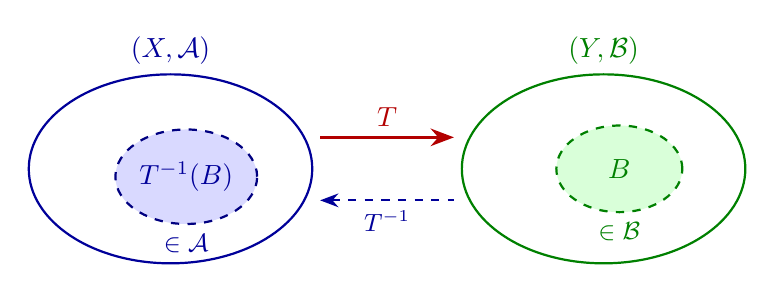
\begin{tikzpicture}[>=Stealth, thick]
  % --- 左側：X ---
  \draw[blue!60!black] (0,0) ellipse (1.8 and 1.2);
  \node[blue!60!black] at (0,1.5) {$(X,\mathcal{A})$};
  % T^{-1}(B)
  \fill[blue!15] (0.2,-0.1) ellipse (0.9 and 0.6);
  \draw[blue!50!black, dashed] (0.2,-0.1) ellipse (0.9 and 0.6);
  \node[blue!60!black] at (0.2,-0.1) {$T^{-1}(B)$};
  \node[blue!60!black, font=\small] at (0.2,-0.95) {$\in\mathcal{A}$};

  % --- 右側：Y ---
  \draw[green!50!black] (5.5,0) ellipse (1.8 and 1.2);
  \node[green!50!black] at (5.5,1.5) {$(Y,\mathcal{B})$};
  % B
  \fill[green!15] (5.7,0.0) ellipse (0.8 and 0.55);
  \draw[green!50!black, dashed] (5.7,0.0) ellipse (0.8 and 0.55);
  \node[green!50!black] at (5.7,0.0) {$B$};
  \node[green!50!black, font=\small] at (5.7,-0.8) {$\in\mathcal{B}$};

  % --- 矢印：T ---
  \draw[->, red!70!black, line width=1.2pt]
    (1.9,0.4) -- node[above] {$T$} (3.6,0.4);
  % --- 矢印：T^{-1} ---
  \draw[<-, blue!60!black, dashed]
    (1.9,-0.4) -- node[below, font=\small] {$T^{-1}$} (3.6,-0.4);
\end{tikzpicture}
\caption{可測写像の概念図．$B\in\mathcal{B}$ の逆像
$T^{-1}(B)$ が $\mathcal{A}$ に属する．}
\label{fig:measurable_map}
\end{figure}

\begin{definition}{押し出し測度}{pushforward}
$(X,\mathcal{A})$，$(Y,\mathcal{B})$ を可測空間，
$\mu$ を $(X,\mathcal{A})$ 上の測度，$T\colon X\to Y$ を可測写像とする．
$T$ による $\mu$ の\textbf{押し出し測度} $T_\#\mu$ を
\[
  T_\#\mu(B) \coloneqq \mu(T^{-1}(B)), \qquad B\in\mathcal{B}
\]
で定義する．
\end{definition}

押し出し測度を用いると，Monge の最適輸送問題は次のように定式化される．

\begin{definition}{Monge 問題}{monge}
$\mathbb{R}^d$ 上の確率測度 $\mu,\,\nu$ と
コスト関数 $c\colon\mathbb{R}^d\times\mathbb{R}^d\to[0,\infty]$ が与えられたとする．
\textbf{Monge 問題}は，$T_\#\mu=\nu$ を満たす可測写像
$T\colon\mathbb{R}^d\to\mathbb{R}^d$（輸送写像）の中で
\[
  \inf_{T:\,T_\#\mu=\nu}\int_{\mathbb{R}^d} c\bigl(x,\,T(x)\bigr)\,d\mu(x)
\]
を達成するものを求める問題である．
\end{definition}

\begin{figure}[ht]
\centering
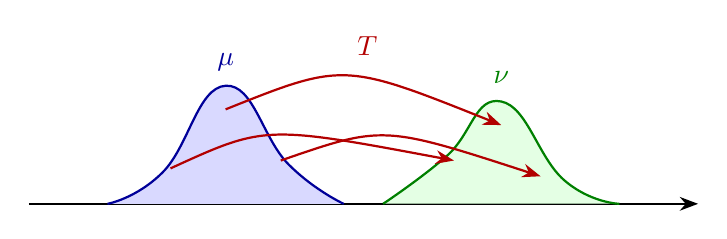
\begin{tikzpicture}[>=Stealth, thick]
  % --- 共通の軸 ---
  \draw[->] (-0.5,0) -- (8,0);

  % --- mu：左寄りの分布 ---
  \fill[blue!15] plot[smooth, tension=0.8]
    coordinates {(0.5,0) (1.2,0.4) (2.0,1.5) (2.8,0.5) (3.5,0)} -- cycle;
  \draw[blue!60!black] plot[smooth, tension=0.8]
    coordinates {(0.5,0) (1.2,0.4) (2.0,1.5) (2.8,0.5) (3.5,0)};
  \node[blue!60!black] at (2.0,1.8) {$\mu$};

  % --- nu：右にずれた分布 ---
  \fill[green!15, opacity=0.7] plot[smooth, tension=0.8]
    coordinates {(4.0,0) (4.8,0.6) (5.5,1.3) (6.3,0.3) (7.0,0)} -- cycle;
  \draw[green!50!black] plot[smooth, tension=0.8]
    coordinates {(4.0,0) (4.8,0.6) (5.5,1.3) (6.3,0.3) (7.0,0)};
  \node[green!50!black] at (5.5,1.6) {$\nu$};

  % --- 輸送写像 T の矢印 ---
  \draw[->, red!70!black] (1.3,0.45) .. controls (2.5,1.0) .. (4.9,0.55);
  \draw[->, red!70!black] (2.0,1.2) .. controls (3.5,1.8) .. (5.5,1.0);
  \draw[->, red!70!black] (2.7,0.55) .. controls (4.0,1.0) .. (6.0,0.35);
  \node[red!70!black] at (3.8,2.0) {$T$};
\end{tikzpicture}
\caption{Monge 問題の概念図．分布 $\mu$ を写像 $T$ によって分布 $\nu$ に移す．}
\label{fig:monge_problem}
\end{figure}

直感的には，$\mu$ が砂山の分布，$\nu$ が穴の分布を表し，
コスト $c(x,y)$ は位置 $x$ の砂を位置 $y$ に運ぶ費用を意味する．
Monge 問題は，砂山をちょうど穴に埋めるための総輸送コストを最小化する
最適な運搬計画を求める問題である．

しかし Monge 問題には，
制約 $T_\#\mu=\nu$ を満たす輸送写像がそもそも存在しない場合がある
という根本的な困難がある．次の例はその典型である．

\begin{example}{Monge 問題の非可解性}{monge_infeasible}
$\mu=\delta_0$（原点に集中するDirac測度），
$\nu=\frac{1}{2}\delta_a+\frac{1}{2}\delta_b$（$a\neq b$）とする．
$T_\#\mu=\nu$ を満たす写像 $T$ が存在するならば，
$T(0)$ は一つの点でなければならないが，
$\nu$ は $a$ と $b$ の二点に測度を分散させている．
写像は1点を2点に分割できないので，
$T_\#\delta_0=\frac{1}{2}\delta_a+\frac{1}{2}\delta_b$
を満たす $T$ は存在しない．
したがって Monge 問題は実行不可能である．
\end{example}

\begin{figure}[h]
\centering
\begin{tikzpicture}[>=Stealth, thick]
  % 左側：mu
  \node[label=above:{$\mu=\delta_0$}] (mu) at (0,0) {};
  \fill (0,0) circle (4pt);
  \node[below=4pt] at (0,0) {測度 $1$};

  % 右側：nu
  \node[label=above:{$\nu$}] at (5,1) {};
  \fill (5,1) circle (3pt);
  \node[right=4pt] at (5,1) {$a$：測度 $\frac{1}{2}$};
  \fill (5,-1) circle (3pt);
  \node[right=4pt] at (5,-1) {$b$：測度 $\frac{1}{2}$};

  % 破線矢印
  \draw[dashed, ->] (0.2,0.1) -- (4.7,0.9);
  \draw[dashed, ->] (0.2,-0.1) -- (4.7,-0.9);

  % 注釈
  \node[draw, rounded corners, fill=yellow!10, font=\small]
    at (2.5,-2) {写像 $T$ は1点を2点に分割できない};
\end{tikzpicture}
\caption{Monge 問題の非可解性（例~\ref{ex:monge_infeasible}）．
$\delta_0$ から $\frac{1}{2}\delta_a+\frac{1}{2}\delta_b$
への輸送写像は存在しない．}
\label{fig:monge_infeasible}
\end{figure}

この例が示すように，Monge 問題は「写像」による輸送を要求するため，
測度の分割が必要な場面で実行不可能になる．
この本質的な制約を克服するため，
Kantorovich は輸送写像を輸送計画（結合測度）に緩和するという着想を導入した．

%% ==========================================================
%%  第2節：Kantorovich 緩和
%% ==========================================================
\section{Kantorovich 緩和}

Kantorovich の着想は，
分布の移動を決定論的な写像 $T$ ではなく，
出発点 $x$ と到着点 $y$ の同時分布 $\pi$ で記述することである．
写像は $x$ から $T(x)$ への一対一の対応を要求するが，
同時分布では $x$ における測度を複数の行き先に分配できるため，
Monge 問題の非可解性の問題を回避できる．

\begin{definition}{輸送計画}{transport_plan}
$\mu,\,\nu$ を $\mathbb{R}^d$ 上の確率測度とする．
$\mathbb{R}^d\times\mathbb{R}^d$ 上の確率測度 $\pi$ が
$\mu$ と $\nu$ の\textbf{輸送計画}であるとは，
$\pi$ の周辺分布がそれぞれ $\mu$ と $\nu$ に一致すること，
すなわち任意のボレル集合 $A,B\subset\mathbb{R}^d$ に対し
\[
  \pi(A\times\mathbb{R}^d) = \mu(A), \qquad
  \pi(\mathbb{R}^d\times B) = \nu(B)
\]
が成り立つことをいう．
$\mu$ と $\nu$ の輸送計画全体の集合を $\Pi(\mu,\nu)$ と記す．
\end{definition}

\begin{definition}{Kantorovich 問題}{kantorovich}
$\mu,\,\nu$ を $\mathbb{R}^d$ 上の確率測度，
$c\colon\mathbb{R}^d\times\mathbb{R}^d\to[0,\infty]$ をコスト関数とする．
\textbf{Kantorovich 問題}は
\[
  \inf_{\pi\in\Pi(\mu,\nu)}
  \int_{\mathbb{R}^d\times\mathbb{R}^d} c(x,y)\,d\pi(x,y)
\]
を求める問題である．
\end{definition}

\begin{remark}{Monge 問題との関係}{monge_kantorovich}
Monge の輸送写像 $T$ は，
$\pi=({\rm id},T)_\#\mu$
（すなわち $\pi(A\times B)=\mu(A\cap T^{-1}(B))$）
という特殊な輸送計画に対応する．
したがって Kantorovich 問題は Monge 問題の真の緩和であり，
Kantorovich 問題の最適値は Monge 問題の最適値以下である．
さらに $\Pi(\mu,\nu)$ は常に非空である——実際，
独立結合 $\pi=\mu\otimes\nu$ は $\Pi(\mu,\nu)$ に属する——ので，
Monge 問題とは異なり Kantorovich 問題は常に実行可能である．
\end{remark}

\begin{theorem}{最小値の存在}{kantorovich_existence}
$c\colon\mathbb{R}^d\times\mathbb{R}^d\to[0,\infty]$ が下半連続であるとする．
このとき Kantorovich 問題の下限は最小値として達成される．
すなわち，ある $\pi^*\in\Pi(\mu,\nu)$ が存在して
\[
  \int_{\mathbb{R}^d\times\mathbb{R}^d} c(x,y)\,d\pi^*(x,y)
  = \inf_{\pi\in\Pi(\mu,\nu)}
    \int_{\mathbb{R}^d\times\mathbb{R}^d} c(x,y)\,d\pi(x,y)
\]
が成り立つ．
\end{theorem}

\begin{proof}
$\Pi(\mu,\nu)$ は周辺分布条件により緊密（tight）であり，
Prokhorov の定理から測度の弱収束に関して相対コンパクトである．
周辺分布条件は弱収束に関して閉じているので，$\Pi(\mu,\nu)$ はコンパクトである．
$c$ が下半連続であることから
$\pi\mapsto\int c\,d\pi$ は弱収束に関して下半連続であり，
コンパクト集合上の下半連続関数は最小値を達成する．
\end{proof}

\begin{theorem}{Kantorovich 双対定理}{kantorovich_duality}
$c\colon\mathbb{R}^d\times\mathbb{R}^d\to[0,\infty]$ が下半連続とする．このとき
\[
  \inf_{\pi\in\Pi(\mu,\nu)}
  \int_{\mathbb{R}^d\times\mathbb{R}^d} c(x,y)\,d\pi(x,y)
  = \sup_{(\varphi,\psi)\in\Phi_c}
  \left(
    \int_{\mathbb{R}^d}\varphi(x)\,d\mu(x)
    + \int_{\mathbb{R}^d}\psi(y)\,d\nu(y)
  \right)
\]
が成り立つ．ここで
$\Phi_c = \{(\varphi,\psi)\in L^1(\mu)\times L^1(\nu)
: \varphi(x)+\psi(y)\le c(x,y)\}$
は\textbf{双対許容対}の集合である．
\end{theorem}

双対問題には明快な経済的解釈がある．
$\varphi(x)$ を出発地 $x$ での積み込み価格，
$\psi(y)$ を到着地 $y$ での荷降ろし価格と考えると，
制約 $\varphi(x)+\psi(y)\le c(x,y)$ は
裁定条件（価格差が輸送コストを超えない）を意味する．
双対問題は，この裁定条件の下で仲介業者の総収入を最大化する問題であり，
強双対性は最適輸送コストと最適価格設定による収入が一致することを述べている．

\begin{remark}{Monge 問題への回帰}{monge_from_kantorovich}
Kantorovich 問題の最適計画 $\pi^*$ が
$\pi^*=({\rm id},T)_\#\mu$ の形に書ける（すなわちグラフ上に集中する）場合，
$T$ は Monge 問題の最適写像でもある．
例えば $c(x,y)=\|x-y\|^2$ かつ $\mu$ が絶対連続のとき，
Brenier の定理により最適輸送写像 $T=\nabla\phi$
（凸関数の勾配）の存在と一意性が保証される．
\end{remark}

\end{document}
